\chapter{SPI sučelje mikrokontrolera STM32L4P5VET6}
	Komponente senzorske pločice FERSAT-a, odnosno analogno-digitalni pretvornik (ADC) ADS131M08 i temperaturni senzori ADT7301 komuniciraju s PDH računalom putem sučelja SPI. S obzirom da se pri razvoju programske potpore PDH računala koriste \textit{Low-Level} biblioteke, za ispravnu implementaciju upravljačkih programa nužno je razumijevanje strukture i načina rada SPI periferije izabranog mikrokontrolera. U nastavku ovog poglavlja dan je općeniti opis SPI protokola i opis SPI periferije porodice mikrokontrolera STM32L4.
	
	\section{SPI protokol}
		\textit{Serial Peripheral Interface} (SPI) sinkrono je serijsko komunikacijsko sučelje, razvijeno u tvrtki Motorola. S obzirom da SPI sučelje omogućava brzinu prijenosa do nekoliko desetaka Mbit/s, obično se koristi za prijenos signala visokih frekvencija između računala ili mikrokontrolera i periferijskih sklopova. Podaci se prenose između jedne upravljačke jedinice \engl{master} i više upravljanih jedinica \engl{slave} korištenjem četiri prijenosne linije: SCLK (\textit{Serial Clock}), MISO (\textit{Master Input Slave Output}), MOSI (\textit{Master Output Slave Input}) i CS (\textit{Chip Select}, ponekad se naziva i \textit{Slave Select}). Signal takta pogoni \textit{master} uređaj, a pomoću linije CS \textit{master} uređaj odabire koji \textit{slave} uređaj smije komunicirati preko linija MISO i MOSI. Slika \ref{fig:spi} prikazuje tipičan način spajanja uređaja SPI sučeljem, u konfiguraciji jednog \textit{master} uređaja i tri \textit{slave} uređaja.
		
		\begin{figure}[htb]
			\centering
			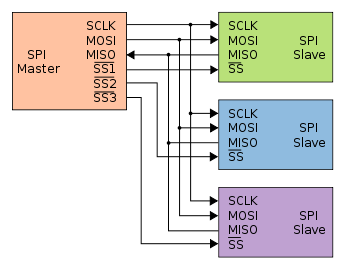
\includegraphics[height=7cm]{slike/spi.png}
			\caption{Povezivanje uređaja SPI sučeljem \cite{spi_wikipedia}}
			\label{fig:spi}
		\end{figure}
	
		Postoje 4 temeljna načina rada \engl{modes} SPI sučelja, a razlikuju se po polaritetu signala takta \engl{Clock Polarity, CPOL} i  načinu čitanja podatka sa strane master uređaja \engl{Clock Phase, CPHA}. CPOL određuje logičku razinu u koju će signal takta poprimiti u neaktivnom stanju \engl{idle state}. CPOL=0 će postaviti nisku razinu, a CPOL=1 visoku. CPHA određuje na koji brid signala takta će \textit{master} uređaj čitati podatak koji se nalazi na liniji. CPHA=0 obično znači da će to biti prvi brid, a CPHA=1 drugi. Ovisno o postavci CPOL, taj brid može biti rastući ili padajući. Ako je CPOL=0 prvi brid će biti rastući, a ako je CPOL=1, prvi brid će biti padajući. Slika \ref{fig:spi_cpol_cpha} prikazuje vremenske odnose za različite postavke CPOL i CPHA.
		
		\begin{figure}[htb]
			\centering
			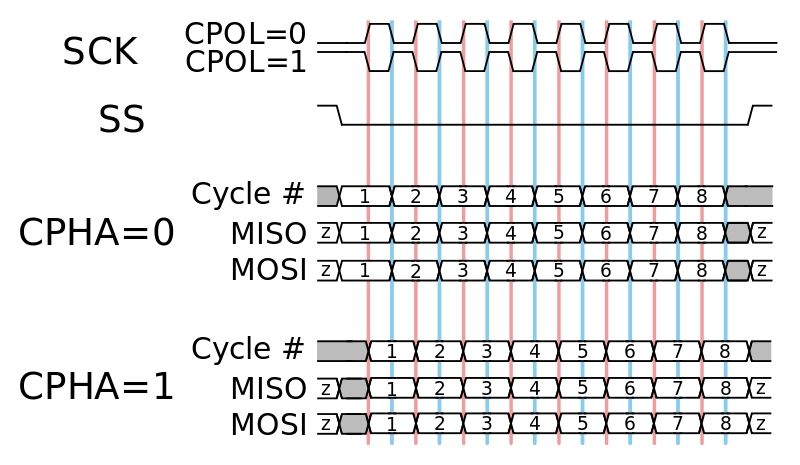
\includegraphics[height=7cm]{slike/spi_cpol_cpha.png}
			\caption{Vremenski dijagram SPI prijenosa s različitim postavkama CPOL i CPHA. Crvene linije označavaju prvi, a plave drugi brid  signala takta. \cite{spi_wikipedia}}
			\label{fig:spi_cpol_cpha}
		\end{figure}
		
	\section{Struktura SPI periferije STM32L4}
		Slika \ref{fig:stm32l4_spi} prikazuje blok dijagram SPI periferije porodice mikrokontrolera STM32L4 \cite{stm32l4_manual}.
	
		\begin{figure}[htb]
			\centering
			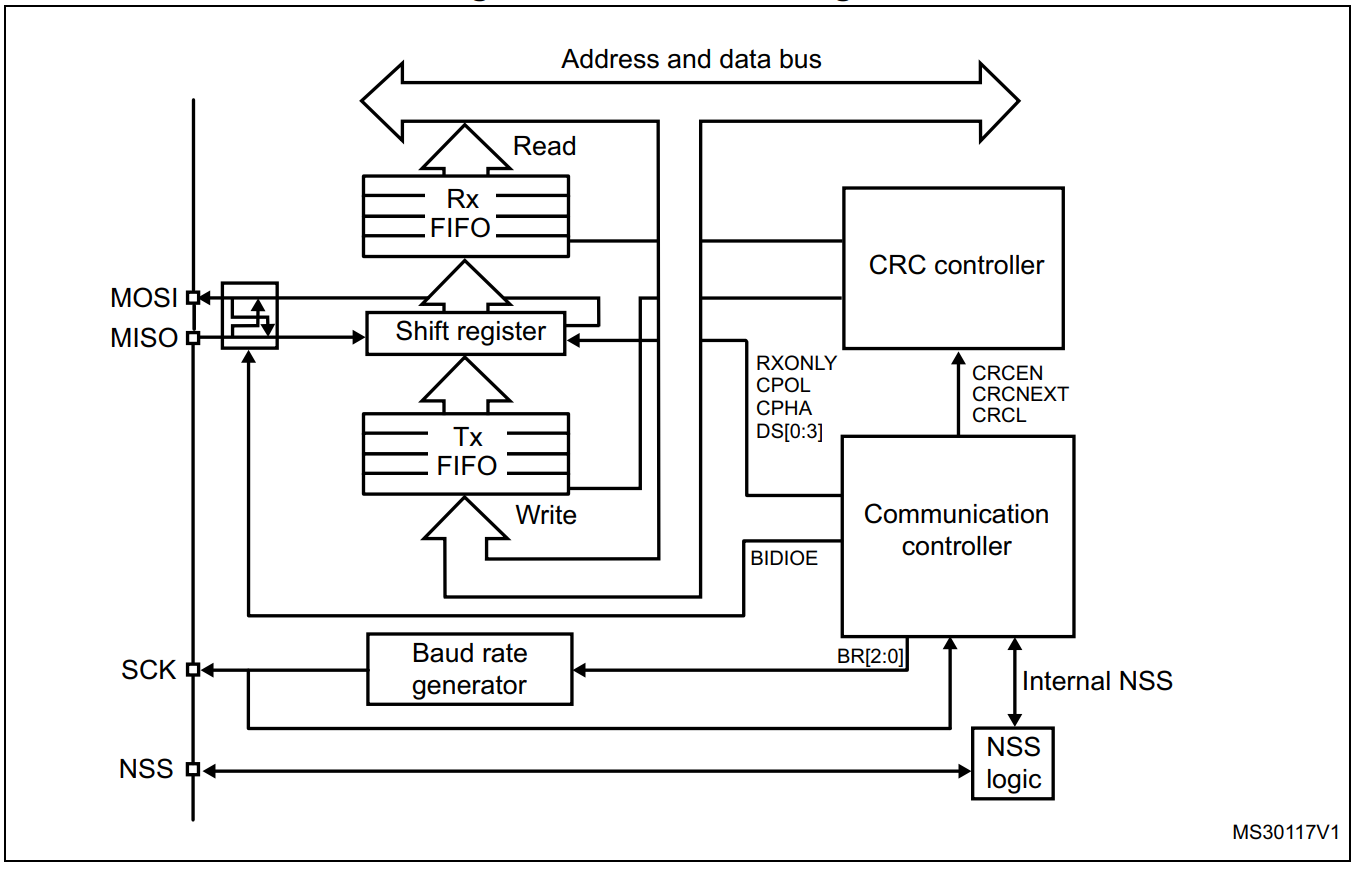
\includegraphics{slike/STM32L4_SPI_blok_dijagram.png}
			\caption{Blok dijagram SPI periferije STM32L4 \cite[str.~1451]{stm32l4_manual}}
			\label{fig:stm32l4_spi}
		\end{figure}
	
		Primanje podataka odvija se na način da riječ koja se prima po MISO liniji prvo ulazi u posmačni registar \engl{shift register}, pri čemu se na svaki period SPI takta posmiče za jedno mjesto. Kada je primljena cijela riječ, ona se na sljedeći brid takta prebacuje na kraj reda Rx FIFO \textit{First In First Out}, pri čemu se postavlja zastavica RXNE (\textit{Receiver Buffer Not Empty}) u registru stanja SPI periferije(SPIx\_SR). Prvom podatku u redu programski se može pristupiti preko SPI podatkovnog registra (SPIx\_DR). Čitanje ovog registra automatski čisti zastavicu RXNE ukoliko je popunjeno manje od četvrtine maksimalnog kapaciteta reda.
		
		Slanje podataka odvija se na sličan način. Riječ upisana u SPIx\_DR sprema se na kraj reda Tx FIFO. Prva riječ u redu prebacuje se u posmačni registar, te se izlazni bit pri svakom posmaku šalje po liniji MOSI. Ako Tx FIFO sadrži manje podataka od pola svog kapaciteta, postavlja se zastavica TXE (\textit{Transmitter Buffer Empty}). Postavljanje te zastavice signalizira programu da se sljedeća riječ može upisati u red.
		
		Važno je naglasiti da SPIx\_DR nije fizički registar, već se radi o virtualnom registru koji služi za pristup redovima Rx FIFO i Tx FIFO. Pisanje u ovaj registar umeće podatak na kraj reda Tx FIFO, a čitanje sadržaja registra vraća prvi podatak u redu Rx FIFO. Oba reda su veličine 32 bita, odnosno mogu primiti 4 8-bitne riječi. Nivo popunjenosti, tj. broj 8-bitnih riječi u redu može se dobiti čitanjem bitova FTLVL[1:0] za Tx FIFO, odnosno FRLVL[1:0] za Rx FIFO u SPIx\_SR. 
		
		SPI kontroler može raditi s duljinama riječi od 4 do 16 bita. U izradi ovog rada korištena je duljina riječi 8 bita.
		
		Kontroler omogućuje hardversko izračunavanje CRC zaštitnog koda. Ova je mogućnost nakon reseta isključena, no može se omogućiti postavljanjem bita CRCEN u registru SPIx\_CR1. Tada će pogreška u prijenosu koju otkrije CRC biti signalizirana postavljanjem zastavice CRCERR u registru SPIx\_SR.
		
	\section{Postupak slanja i primanja podataka}
		%TODO: inicijalizacija?
		
		SPI sučelje može funkcionirati u nekoliko načina rada s obzirom na smjer komunikacije. Ti načini rada su: \textit{Full Duplex Master, Full Duplex Slave, Half Duplex Master, Half Duplex Slave, Simplex Receive Only} i \textit{Simplex Transmit Only}. U upravljačkim programima izrađenim u sklopu ovog rada korišten je način rada \textit{Full Duplex Master}, pa će zato u nastavku ovog potpoglavlja biti opisan postupak kojeg upravljački program mora izvršiti za ispravnu komunikaciju u tom načinu rada.
		
		Važno je naglasiti da je u \textit{Full Duplex Master} načinu rada signal SPI takta određen slanjem podataka. SPI kontroler počinje generirati signal takta upisom prve riječi podatka u podatkovni registar, te nastavlja generirati signal takta dok sve riječi nisu poslane. Ako je zadnja riječ poslana i nema novih riječi u redu Tx FIFO, kontroler prestaje s generiranjem takta do sljedećeg upisa u podatkovni registar. \\
		
		Upravljački program mora slijediti sljedeću proceduru\footnote{Ova procedura je prilagođena verzija procedure opisane u priručniku mikrokontrolerske porodice STM32F4 \cite[str.~887]{stm32f4_manual}.}:
		\begin{enumerate}
			\item Omogućiti SPI postavljanjem bita SPE u registru SPIx\_CR1.
			\item Upisati prvu riječ za slanje u podatkovni registar.
			\item Čekati dok se ne postavi zastavica TXE i zatim upisati sljedeću riječ u podatkovni registar. Čekati dok se ne postavi zastavica RXNE i zatim pročitati riječ iz podatkovnog registra. Ponavljati ovaj korak do (uključivo) predzadnje pročitane riječi.
			\item  Čekati dok se ne postavi zastavica RXNE i pročitati zadnju riječ iz podatkovnog registra.
		\end{enumerate}
	
		Čekanje zastavice TXE prilikom upisa druge riječi nije obavezno jer će ona sigurno biti postavljena, odnosno Tx FIFO sigurno može primiti dvije 8-bitne riječi. Međutim, čekanje je potrebno za svaki sljedeći upis.

		Gornja procedura implementirana je funkcijom \texttt{SPI\_TransmitReceive()}, koja pruža praktično sučelje za SPI prijenos po uzoru na HAL biblioteke.

		\begin{lstlisting}
		void SPI_TransmitReceive(SPI_TypeDef *SPIx, uint8_t len, uint8_t *tx_buffer, uint8_t *rx_buffer) 
		{
			LL_SPI_Enable(SPIx);
			
			LL_SPI_TransmitData8(SPIx, tx_buffer[0]);
			for (int i = 0; i < len - 1; i++) {
				while ( !LL_SPI_IsActiveFlag_TXE(SPIx) );
				LL_SPI_TransmitData8(SPIx, tx_buffer[i + 1]);
				while ( !LL_SPI_IsActiveFlag_RXNE(SPIx) );
				rx_buffer[i] = LL_SPI_ReceiveData8(SPIx);
			}
			
			while ( !LL_SPI_IsActiveFlag_RXNE(SPIx) );
			rx_buffer[len - 1] = LL_SPI_ReceiveData8(SPIx);
		}
		\end{lstlisting}
	
		Ako je nakon dovršenog SPI prijenosa potrebno staviti mikrokontroler u način rada male potrošnje, tada treba na ispravan način onemogućiti SPI. U nekim drugim SPI načinima rada potrebno je onemogućiti SPI nakon svakog prijenosa, npr. ako u \textit{Receive Only Master} načinu rada mikrokontroler komunicira sa sklopom koji kontinuirano šalje podatke, kako bi se spriječilo slanje dodatnih neželjenih podataka. U \textit{Full Duplex} načinu rada to obično nije potrebno, međutim dobra je praksa slijediti pravilnu proceduru za onemogućavanje SPI sučelja nakon završetka prijenosa kako bi se spriječila korupcija zadnje poslane riječi. Procedura za onemogućavanje je:
		
		\begin{enumerate}
			\item Čekati dok se ne isprazni odlazni red (TX FIFO) provjerom bitova FTLVL[1:0] u SPI statusnom registru.
			\item Čekati dok se ne spusti zastavica BSY u SPI statusnom registru.
			\item Onemogućiti SPI čišćenjem bita SPE u registru CR1.
		\end{enumerate}
		
		Tijekom uhodavanja SPI komunikacije sa sklopom ADT7301 uočena je greška u implementaciji HAL biblioteke za rad s SPI periferijom kada je SPI u \textit{Receive Only} načinu rada. Naime, u navedenom načinu rada potrebno je očistiti SPE bit točno jedan ciklus SPI takta nakon primitka predzadnje riječi kako bi se spriječilo da uređaj koji šalje podatak inicira prijenos nove riječi \cite[str.~894]{stm32f4_manual}. HAL funkcija \texttt{HAL\_SPI\_TransmitReceive()} čisti SPE bit tek nakon primitka zadnje riječi, zbog čega senzor šalje još jednu riječ, pa ukupna duljina prijenosa iznosi 24 bita umjesto 16. Također, funkcija čeka da se sklopovski očisti zastavica RXNE prije nego što završi s izvođenjem, a s obzirom da se zadnja riječ nikad ne pročita, zastavica uvijek ostaje postavljena. Zbog toga funkcija uvijek čeka do isteka \textit{timeout} intervala, što nije poželjno ponašanje. No, to nije predstavljalo problem u daljnem tijeku izrade ovog rada, jer su za razvoj korištene LL biblioteke i \textit{Full Duplex} način rada.
		
	\section{Prijenos podataka korištenjem DMA sklopa}
		
		Prijenos podataka SPI sučeljem između PDH računala i AD pretvornika podrazumijeva slanje relativno velike količine podataka, što može prilično dugo trajati, ovisno o brzini prijenosa. Zato je korisno koristiti DMA (\textit{Direct Memory Access}) sklop za prijenos podataka između SPI periferije i memorije. Za vrijeme DMA prijenosa procesor je rasterećen pa može obavljati druge korisne zadatke, odnosno moguće je ostvarenje neblokirajućih funkcija za SPI prijenos. Dodatna prednost je i smanjenje ukupnog trajanja komunikacije. Naime, kada se SPI komunikacija obavlja programski, program mora prvo upisati odlaznu riječ u podatkovni registar, zatim čekati primitak cijele dolazne riječi, te pročitati riječ prije upisa sljedeće riječi. To ponekad može uzrokovati diskontinuirani prijenos, odnosno periode čekanja između slanja dvije riječi. \cite[str.~890]{stm32f4_manual} Korištenjem DMA slanje i primanje može se obavljati istovremeno, što eliminira ovaj problem.
		
		Odabrani mikrokontroler sadrži dva DMA sklopa, a svaki od njih ima 7 prijenosnih kanala. Periferija SPI3 spojena je na sklop DMA2, i to tako da je linija zahtjeva za dolazni prijenos (RX) spojena na kanal 1, a odlazni prijenos (TX) na kanal 2. 
		
		Prije korištenja DMA sklopa potrebno je obaviti određenu inicijalizaciju. Većina te inicijalizacije, kao što je omogućavanje prekida, postavljanje smjera prijenosa i slično, može se obaviti u alatu CubeMX, pa će ovdje biti opisani samo oni koraci koji se moraju obaviti nakon CubeMX inicijalizacije, s obzirom da su oni posebno važni za razvoj programske potpore. Ne smije se zaboraviti ni inicijalizacija SPI periferije, kako bi ona mogla slati zahtjeve za DMA prijenos. Potrebni koraci su:
		\begin{enumerate}
			\item Postaviti adresu periferije za svaki kanal upisom u registar CPAR. Ova se adresa neće inkrementirati nakon svakog prijenosa.
			\item Postaviti adresu memorije za svaki kanal upisom u registar CMAR. Ova će adresa biti inkrementirana nakon svakog prijenosa, a iznos inkrementa ovisi o veličini riječi.
			\item Omogućiti \textit{Transfer Complete} (TC) prekide za svaki kanal upisom bita TCIE u registru CCR.
			\item Postaviti duljinu prijenosa, odnosno broj riječi koje se trebaju prenijeti za svaki kanal upisom u registar CNDTR.
			\item Omogućiti SPI RX zahtjeve za DMA prijenos upisom bita RXDMAEN u SPI registru CR2.
			\item Omogućiti odgovarajuće DMA kanale upisom bita EN u registru CCR za svaki kanal.
			\item Omogućiti SPI TX zahtjeve za DMA prijenos upisom bita TXDMAEN u SPI registru CR2.
			\item Omogućiti prekide koje okidaju SPI zastavice RXNE i TXE upisom bitova RXNEIE odnosno TXEIE u SPI registru CR2.
		\end{enumerate}
		
		Po završetku DMA prijenosa za svaki kanal, bit će generiran \textit{Transfer Complete} (TC) prekid. Bitno je primijetiti da se prekid generira za svaki kanal posebno. U prekidnoj rutini tih prekida potrebno je očistiti zastavicu CTCFIFx (za kanal x) u DMA registru IFCR i onemogućiti odgovarajući kanal kako bi se spriječio nastavak prijenosa na sljedeći SPI zahtjev kada se postavi zastavica TXE ili RXNE. Kada završe oba prekida, potrebno je onemogućiti SPI RX i TX DMA zahtjeve. Ako se želi pokrenuti novi prijenos, potrebno je ponoviti korake 4 do 8 gore opisane procedure.
		
		